\begin{savequote}[45mm]
\ascii{Any fool can write code that a computer can understand. Good programmers write code that humans can understand.}
\qauthor{\ascii{- Martin Flower}}
\end{savequote}

\chapter{队列} 
\label{ch:queue}

\begin{content}

\ascii{TensorFlow}的\code{Session}是线程安全的。也就是说,多个线程可以使用同一个\code{Session}实例,并发地执行同一个图实例的不同\ascii{OP};\ascii{TensorFlow}执行引擎会根据输入与输出对图实施剪枝,得到一个最小依赖的子图。

因此,通过多线程并使用同一个\code{Session}实例,并发地执行同一个图实例的不同\ascii{OP},最终实现的效果是子图之间的并发执行。

对于典型的模型训练,可以充分发挥\code{Session}多线程的并发能力,提升训练的性能。例如,输入子图运行在一个单独的线程中,用于准备样本数据;而训练子图则运行在另外一个单独的线程中,并按照\code{batch\_size}的大小一个批次取走训练样本,并启动迭代的训练过程。

本文将讲解上述并发模型中的基础设施,包括队列,多线程的协调器,及其控制\code{Enqueue OP}执行的\ascii{QueueRunner}。

\end{content}

\section{队列}

\begin{content}

在\ascii{TensorFlow}的执行引擎中,\ascii{Queue}是一种控制异步计算的强大工具。特殊地,\ascii{Queue}是一种特殊的\ascii{OP},与\ascii{Variable}类似,它是一类有状态的\ascii{OP}。

与之类似,\ascii{Variable}拥有关联的\ascii{Assign}等修改其状态的\ascii{OP},\ascii{Queue}也有与之关联的\ascii{OP},例如\code{Enqueue,Dequeue,EnqueueMany,DequeueMany}等\ascii{OP},它们都能直接修改\ascii{Queue}的状态。

\subsection{FIFOQueue}

举一个简单例子。首先,构造了一个\code{FIFOQueue}队列;然后,在计算图中添加了一个\code{EnqueueMany},该\ascii{OP}用于在队列头部追加\ascii{1}个或多个元素;其次,再添加一个出队的\code{Dequeue};最后,将出队元素的值增加\ascii{1},再将其结果入队。在启动计算图执行之前,计算图的构造如下图所示。

\begin{figure}[!h]
\centering
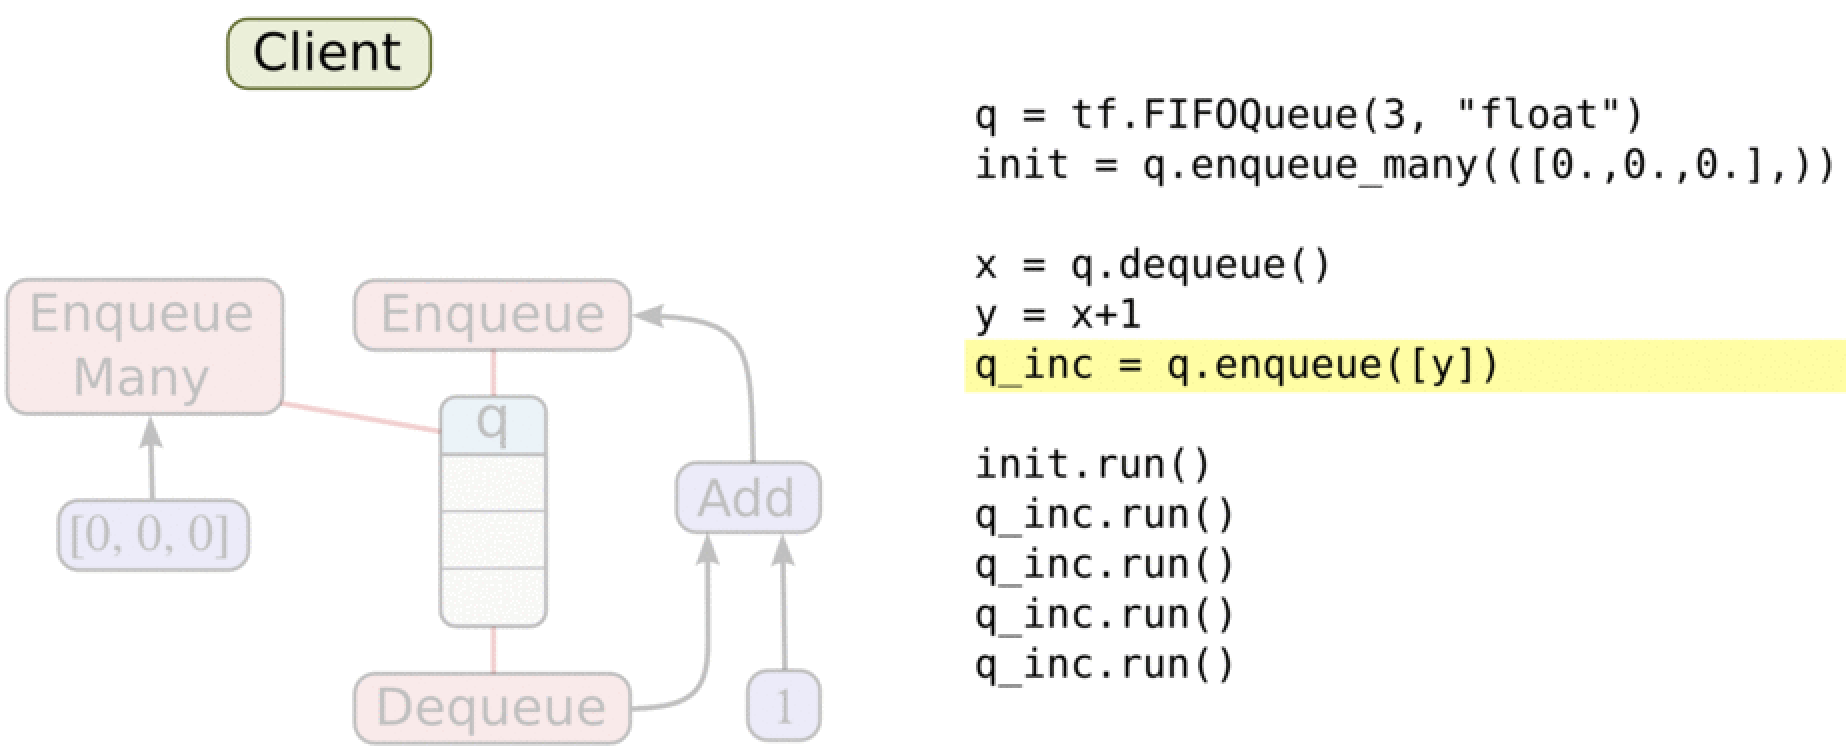
\includegraphics[width=0.9\textwidth]{figures/py-queue-example-1.png}
\caption{图构造期}
 \label{fig:py-queue-example-1}
\end{figure}

执行\code{EnqueueMany}操作后,计算图的状态如下图所示。

\begin{figure}[!h]
\centering
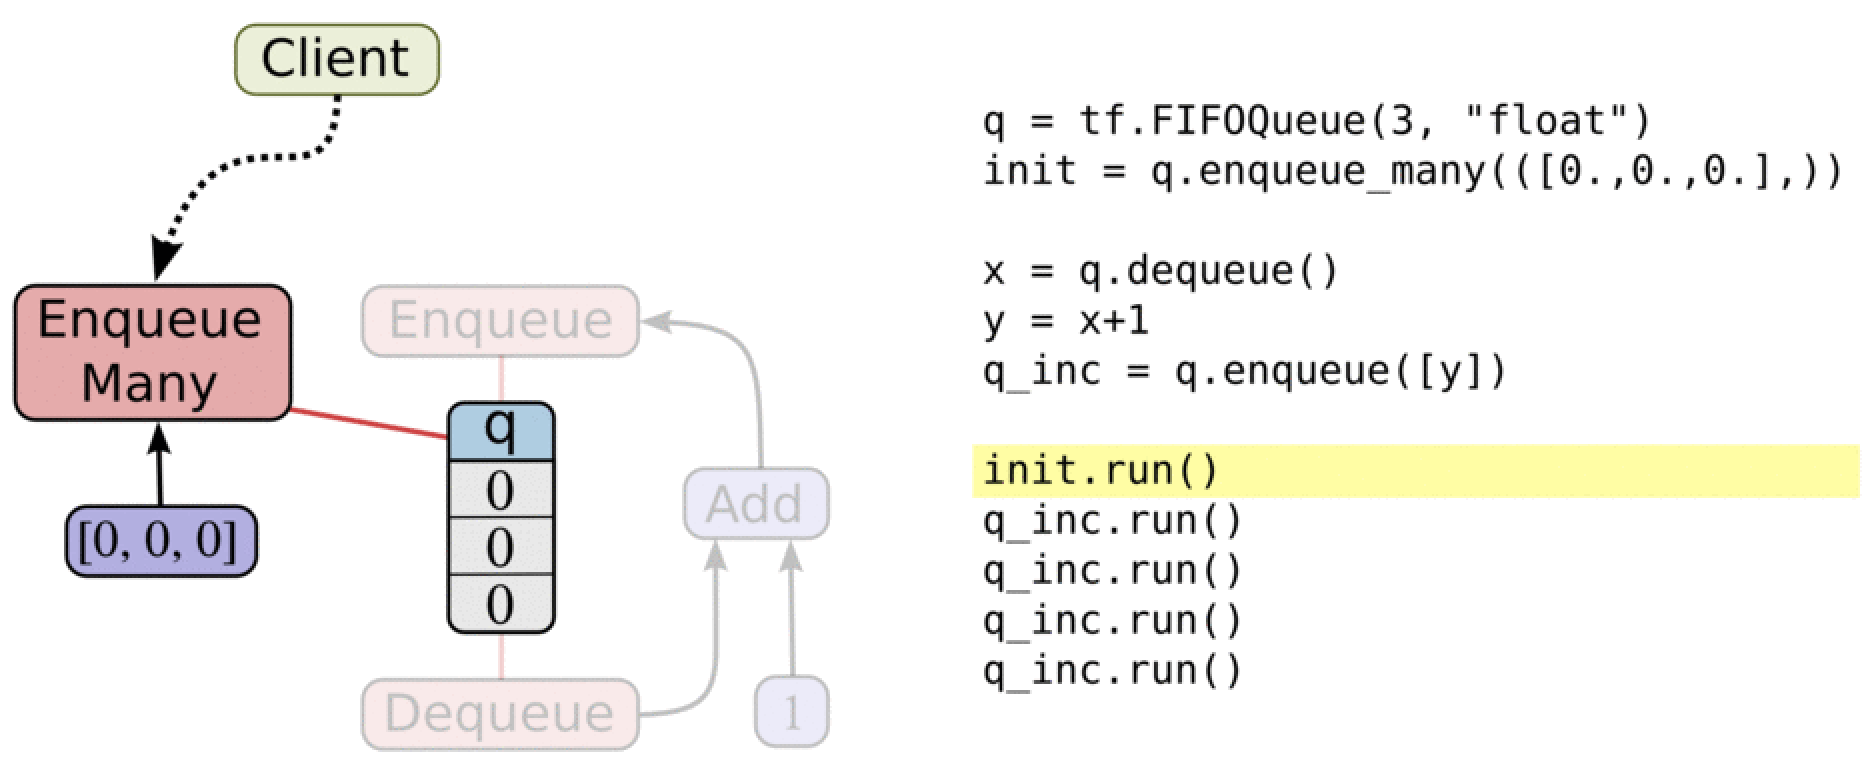
\includegraphics[width=0.9\textwidth]{figures/py-queue-example-2.png}
\caption{图执行期:执行一次EnqueueMany}
 \label{fig:py-queue-example-2}
\end{figure}


执行第一步\code{Enqueue}后,计算图的状态如下图所示。

\begin{figure}[!h]
\centering
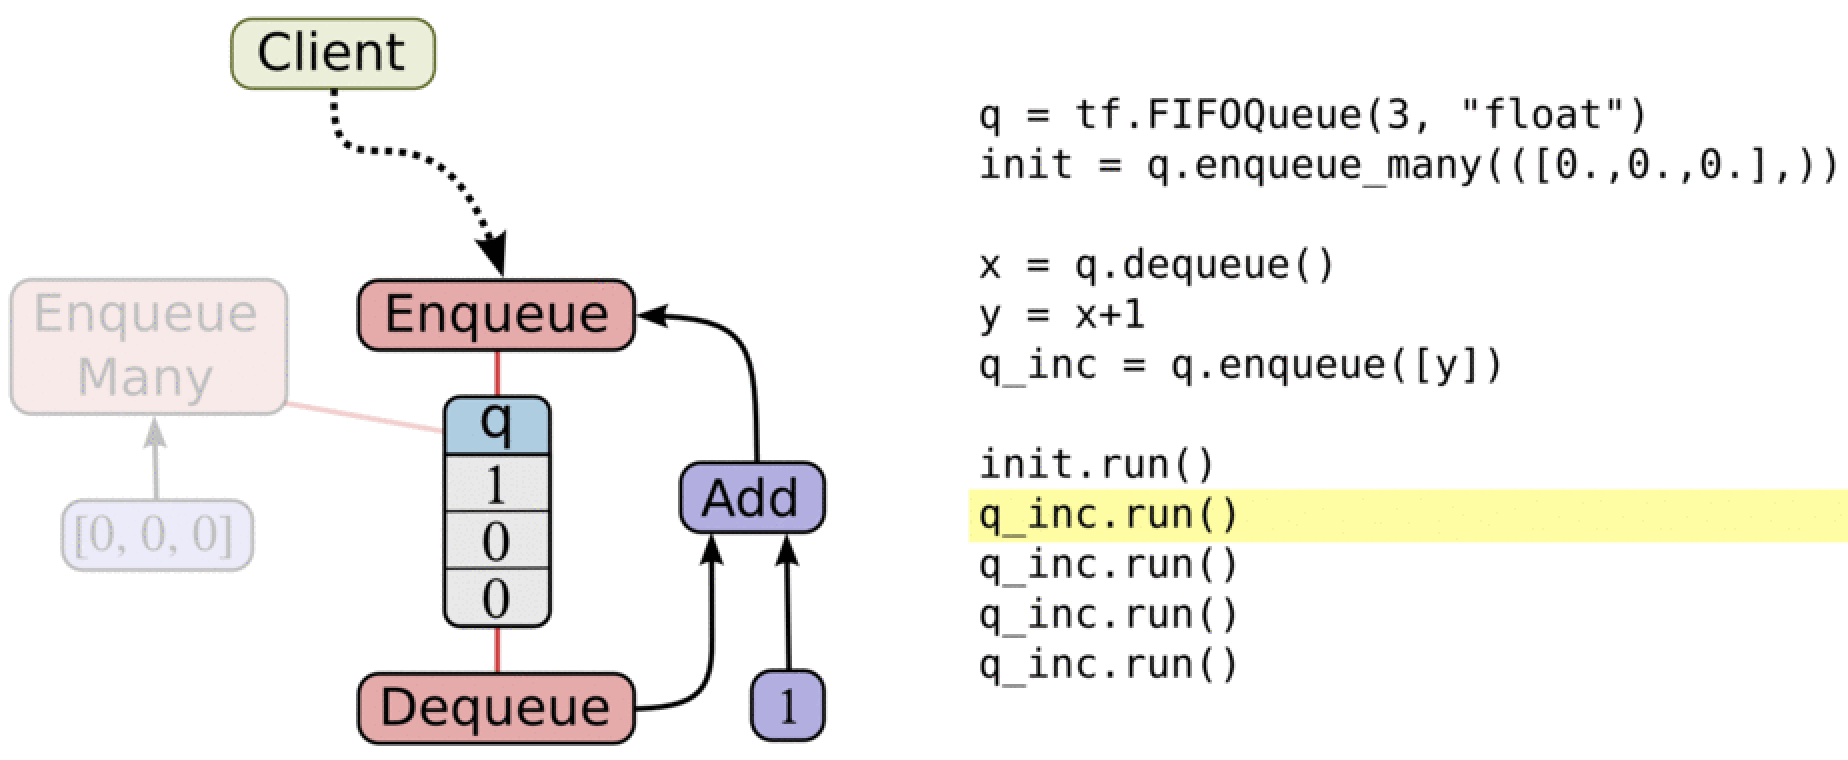
\includegraphics[width=0.9\textwidth]{figures/py-queue-example-3.png}
\caption{图执行期:执行一次Enqueue}
 \label{fig:py-queue-example-3}
\end{figure}

\subsection{用途}

队列在模型训练中扮演重要角色,后文将讲述数据加载的\ascii{Pipeline},训练模型常常使用\code{RandomShuffleQueue}为其准备样本数据。为了提高\ascii{IO}的吞吐率,可以使用多线程,并发地将样本数据追加到样本队列中;与此同时,训练模型的线程迭代执行\code{train\_op}时,一次获取\code{batch\_size}大小的批次样本数据。

显而易见,队列在\ascii{Pipeline}过程中扮演了异步协调和数据交换的功能,这给\ascii{Pipeline}的设计和实现带来很大的弹性空间。

需要注意的是,为了使得队列在多线程最大化发挥作用,需要解决两个棘手的问题:

\begin{enum}
  \eitem{如何同时停止所有的线程,及其处理异常报告?}
  \eitem{如何并发地向队列中追加样本数据?} 
\end{enum}

因此,\ascii{TensorFlow}设计了\code{tf.train.Coordinator}和\code{tf.train.QueueRunner}两个类,分别解决上述两个问题。

这两个类相辅相成,\code{Coordinator}协调多个线程同时停止运行,并且向等待停止通知的主程序报告异常;而\code{QueueRunner}创建了一组线程,并协作多个入队\ascii{OP}(例如\code{Enqueue,EnqueueMany})的执行。

\end{content}

\section{协调器}

\begin{content}

\code{Coordinator}提供了一种同时停止一组线程执行的简单机制。它拥有\ascii{3}个重要的方法:

\begin{enum}
\eitem{\code{should\_stop}: 判断当前线程是否应该退出}
\eitem{\code{request\_stop}: 请求所有线程停止执行}
\eitem{\code{join}: 等待所有线程停止执行}
\end{enum}

\subsection{使用方法}

一般地,主程序常常使用如下模式使用\code{Coordinator}。

\begin{leftbar}
\begin{python}
# Create a coordinator.
coord = tf.train.Coordinator()

# Create 10 threads that run 'MyLoop()'
threads = [threading.Thread(target=MyLoop, args=(coord,)) 
          for i in xrange(10)]

# Start the threads.
for t in threads:
  t.start()
  
# wait for all of them to stop
coord.join(threads)
\end{python}
\end{leftbar}

任何子线程,都可以通过调用\code{coord.request\_stop},通知其他线程停止执行。因此,每个线程的迭代执行中,都要事先检查\code{coord.should\_stop()}。一旦\code{coord.request\_stop}被调用,其他线程的\code{coord.request\_stop()}将立即返回\code{True}。

一般地,一个子线程的迭代执行方法遵循如下实现模式。

\begin{leftbar}
\begin{python}
def MyLoop(coord):
  try
    while not coord.should_stop():
      # ...do something...
  except Exception as e:
    coord.request_stop(e)
\end{python}
\end{leftbar}

\subsection{异常处理}

当某个线程发生了异常,则可以通过\code{coord.request\_stop(e)}报告异常的发生。

\begin{leftbar}
\begin{python}
try:
  while not coord.should_stop():
    # ...do some work...
except Exception as e:
  coord.request_stop(e)
\end{python}
\end{leftbar}

为了消除异常代码处理的重复代码,可以使用\code{coord.stop\_on\_exception()}的上下文管理器。

\begin{leftbar}
\begin{python}
with coord.stop_on_exception():
  while not coord.should_stop():
    # ...do some work...
\end{python}
\end{leftbar}

其中,该异常也会在\code{coord.join}中被重新抛出。因此,在主程序也需要合理地处理异常。

\begin{leftbar}
\begin{python}
try:
  # Create a coordinator.
  coord = tf.train.Coordinator()

  # Create 10 threads that run 'MyLoop()'
  threads = [threading.Thread(target=MyLoop, args=(coord,)) 
            for i in xrange(10)]

  # Start the threads.
  for t in threads:
    t.start()

  # wait for all of them to stop
  coord.join(threads)
except Exception as e:
  # ...exception that was passed to coord.request\_stop(e)
\end{python}
\end{leftbar}

\subsection{实战:LoopThread}

\end{content}

\section{QueueRunner}

\begin{content}

一个\code{QueueRunner}实例持有一个或多个\code{Enqueue}的入队\ascii{OP},它为每个\code{Enqueue OP}启动一个线程。

\begin{figure}[!htbp]
\centering
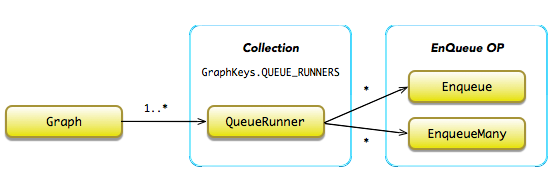
\includegraphics[width=0.9\textwidth]{figures/tf-queue-runner-model.png}
\caption{TensorFlow系统架构}
 \label{fig:tf-queue-runner-model}
\end{figure}

\subsection{注册QueueRunner}

可以调用\code{tf.train.add\_queue\_runner}往计算图中注册\code{QueueRunner}实例,并且将其添加到\code{GraphKeys.QUEUE\_RUNNERS}集合中。

\begin{leftbar}
\begin{python}
def add_queue_runner(qr, collection=ops.GraphKeys.QUEUE_RUNNERS):
  ops.add_to_collection(collection, qr)
\end{python}
\end{leftbar}

\subsection{执行QueueRunner}

可以调用\code{tf.train.start\_queue\_runners}时,它会从计算图中找到所有\code{QueueRunner}实例,并从\code{QueueRunner}实例中取出所有\code{Enqueue OP},为每个\ascii{OP}启动一个线程。

\begin{leftbar}
\begin{python}
def start_queue_runners(sess, coord, daemon=True, start=True,
                        collection=ops.GraphKeys.QUEUE_RUNNERS):
  with sess.graph.as_default():
    threads = []
    for qr in ops.get_collection(collection):
      threads.extend(qr.create_threads(
          sess, coord=coord, daemon=daemon, start=start))
  return threads
\end{python}
\end{leftbar}

在\code{QueueRunner.create\_threads}方法中,为其包含的每个\code{Enqueue}类型的\ascii{OP}启动单独的线程。

\begin{leftbar}
\begin{python}
class QueueRunner(object):
  def create_threads(self, sess, coord, daemon, start):
    """Create threads to run the enqueue ops.
    """
    threads = [threading.Thread(
        target=self._run, args=(sess, op, coord))
        for op in self._enqueue_ops]
    if coord:
      threads.append(threading.Thread(
          target=self._close_on_stop, 
          args=(sess, self._cancel_op, coord)))
    for t in threads:
      if coord:
        coord.register_thread(t)
      if daemon:
        t.daemon = daemon
      if start:
        t.start()
    return threads
\end{python}
\end{leftbar}

\subsubsection{迭代执行Enqueue}

每个\code{Enqueue}子线程将迭代执行\code{Enqueue OP}。当发生\code{OutOfRangeError}异常时,将自动关闭队列,并退出子线程;但是,如果发生其他类型的异常,会主动通知\code{Coordinator}停止所有线程的运行,并退出子线程。

\begin{leftbar}
\begin{python}
class QueueRunner(object):
  def _run(self, sess, enqueue_op, coord):
    try:
      enqueue_callable = sess.make_callable(enqueue_op)
      while True:
        if coord.should_stop():
          break
        try:
          enqueue_callable()
        except errors.OutOfRangeError:  
          sess.run(self._close_op)
          return
    except Exception as e:
      coord.request_stop(e)
\end{python}
\end{leftbar}

\subsubsection{监听队列关闭}

另外,如果给定\code{Coordinator}实例,\code{QueueRunner}还会额外启动一个线程;当\code{Coordinator}实例被触发调用\code{request\_stop}方法后,该线程将会自动关闭队列。

\begin{leftbar}
\begin{python}
class QueueRunner(object):
  def _close_on_stop(self, sess, cancel_op, coord):
    """Close the queue, and cancel pending enqueue ops
       when the Coordinator requests stop.
    """
    coord.wait_for_stop()
    try:
      sess.run(cancel_op)
    except Exception:
      pass
\end{python}
\end{leftbar}

其中,\code{Queue}的\code{Cancel OP}与\code{Close OP}都会关闭队列,但是\code{Cancel OP}会撤销已缓存的\code{Enqueue OP}列表,但\code{Close OP}则保留已缓存的\code{Enqueue OP}列表。

\subsection{关闭队列}

当队列被关闭后,对于任何尝试\code{Enqueue}将会产生错误。但是,对于任何尝试\code{Dequeue}依然是成功的,只要队列中遗留元素;否则,\code{Dequeue}将立即失败,抛出\code{OutOfRangeError}异常,而不会阻塞等待更多元素被入队。
